\documentclass[letterpaper]{article}
\usepackage{geometry}
\geometry{letterpaper, portrait, margin=.8in,top=1in}
\usepackage[english]{babel}
\usepackage[utf8]{inputenc}
\usepackage{amsmath}
\usepackage{graphicx}
\usepackage[backend=biber]{biblatex}
\usepackage{hyperref}
\usepackage{listings}
\usepackage{color}
\definecolor{dkgreen}{rgb}{0,0.6,0}
\definecolor{gray}{rgb}{0.5,0.5,0.5}
\definecolor{mauve}{rgb}{0.58,0,0.82}
\lstset{frame=tb,
  language=C++,
  aboveskip=3mm,
  belowskip=3mm,
  showstringspaces=false,
  columns=flexible,
  basicstyle={\small\ttfamily},
  numbers=none,
  numberstyle=\tiny\color{gray},
  keywordstyle=\color{blue},
  commentstyle=\color{dkgreen},
  stringstyle=\color{mauve},
  breaklines=true,
  breakatwhitespace=true,
  tabsize=3
}
\bibliography{ROOT0908}
\title{Using Trees in ROOT}
\author{Jason Wyenberg}
\begin{document}
\maketitle
\begin{abstract}
I demonstrate how to create a Tree file and read a histogram from it, and then plot some data.
\end{abstract}
\section{Trees with ROOT}
\subsection{Creating a Tree and Working with the Data}
The following code was written as a script for Root:
\begin{lstlisting}
// C file that builds a tree and generates a histogram of the dm data from Jing's oil.dat file

void oil(){

//Declare variables

  Char_t   date[11];
  Int_t    dd;
  Int_t    milage;
  Int_t    dm;
  Float_t  daily;

//Create new files
  TFile *f = new TFile("oil.root","RECREATE");
  
  FILE *fp = fopen("oil.dat","r");
//fopen opens oil.dat. "r" means read and write
  
  TTree *tree = new TTree("T","Jing's Oil data");
  tree->Branch("date",&date,"date/C");
  tree->Branch("dd",&dd,"dd/I");
  tree->Branch("milage",&milage,"milage/I");
  tree->Branch("dm",&dm,"dm/I");
  tree->Branch("daily",&daily,"daily/F");
  char line[40];    //number of entries must be greater than the amount of lines
  while (fgets(&line,40,fp)) {
    sscanf(&line[0], "%s %d %d %d %g",&date,&dd,&milage,&dm,&daily);
    tree->Fill();
  }
  
  tree->Print();
  tree->Write();
  
  TCanvas *can = new TCanvas;
  can->Divide(2,2);
  can->cd(1);
  T->Draw("dd:dm:daily","daily<100","colz");
  
  TH1F *hdm = new TH1F("hdm",";daily milage", 10, 0, 8500);

  int n = (Int_t)T->GetEntries();
  for (Int_t i=0; i<n; i++)  {
    T->GetEntry(i);
    hdm->Fill(dm);
  }
  
  can->cd(2);
  hdm->Draw();
  
  can->cd(3);
  hdm->Draw("e");
  
  TF1 *fc = new TF1("fc","[3]*x+gaus(0)",0,8500);
  fc->SetParameters(13.,4000.,4000.,.00025);
  fc->SetLineColor(kMagenta);
  TGraph *gr = new TGraph(hdm);
  gr->SetTitle("Fit");
  gr->Fit("fc");
  gr->Draw("a*");
  
  hdm->Print();
  hdm->Write();
  
}
\end{lstlisting}
The result was the plots shown in Figure \ref{Oil_data}.
\begin{figure}[htpb]
  \centering
  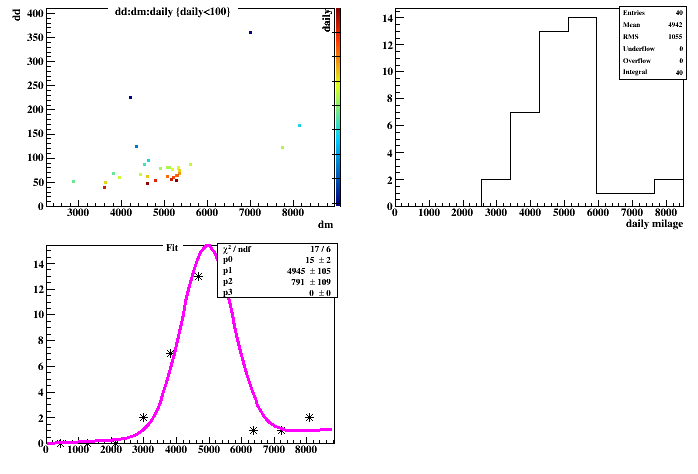
\includegraphics[width=.8\linewidth]{Oil_data}
  \caption{Data from Tree}
  \label{Oil_data}
\end{figure}
\newpage
\printbibliography 
\end{document}
